\documentclass[]{scrartcl}

\usepackage{amsmath}
\usepackage{amssymb}
\usepackage[utf8]{inputenc}
\usepackage[T1]{fontenc}
\usepackage{lmodern}
\usepackage{ngerman}
\usepackage{geometry}
\usepackage{graphicx}
\usepackage{wrapfig}
\usepackage{caption}
\usepackage{wasysym}
\usepackage{siunitx}
\usepackage{picinpar}
\usepackage{tikz}
\usepackage{float}
\usepackage{mathtools}


\renewcommand{\figurename}{Abb.}
\usepackage[
	colorlinks=true,
	urlcolor=blue,
	linkcolor=black
]{hyperref}


%Hier Titel und so
\newcommand{\versuchnummer}{V21} 
\newcommand{\versuchname}{Optisches Pumpen} 
\newcommand{\versuchdatum}{04.07.2016} 


\title{Versuch \versuchnummer\\ \versuchname}
\subtitle{Physikalisches Fortgeschrittenenpraktikum}
\author{Robert Rauter und Björn Lindhauer}
\date{\versuchdatum} 
\begin{document}
\begin{titlepage}
{\large \versuchdatum}
\vspace{7cm}
\begin{center}
\textbf{\huge Versuch \versuchnummer}\\
\vspace{0.5cm}
\textbf{\huge \versuchname}\\
\vspace{0.2cm}
\textbf{ Physikalisches Fortgeschrittenenpraktikum}\\
\vspace{9cm}

{\Large Robert Rauter \ \ \hspace{1.5cm} und \hspace{1.5cm} Björn Lindhauer}\\
{ \url{robert.rauter@tu-dortmund.de} \ \ \hspace{2cm} \url{bjoern.lindhauer@tu-dortmund.de}}
\end{center}
\end{titlepage}
\section{Einleitung}
In diesen Versuch sollen die Landéschen $g$-Faktoren, der Spins der Elektronenhülle und der Spin des Kerns der stabilen Rubidium-Isotope $\prescript{85}{}{\text{Rb}}$ und $\prescript{87}{}{\text{Rb}}$ bestimmt werden.
\section{Theoretische Grundlagen}
Nach dem Aufbauprinzip von Bohr besitzt jedes Atom Elektronenhüllen, welche definierte Energieniveaus besitzen. Es werden zunächst die inneren Niveaus unter der Berücksichtigung des Paul-Prinzips voll besetzt. Ist die äußerste Schale nicht voll besetzt und befindet sich das Atom im thermischen Gleichgewicht, so folgt die Besetzung der Niveaus der äußeren Schale einer Boltzmann-Verteilung gemäß der statistischen Physik.\\
Es lässt sich somit das Besetzungsverhältnis zweier Zustände mit den Energien $W_1$ und $W_2$ durch
\begin{align}
\frac{N_2}{N_1}=\frac{g_2}{g_1}\frac{\exp\left(-\beta W_2\right)}{\exp\left(-\beta W_2\right)}\label{eq:besetzungsverhaeltnisthermisch}
\end{align}
bestimmen. Die $g_i$ sind dabei statistische Gewichte, die die Zahl der Niveaus mit Energie $W_i$ angibt.
\subsection{Ziel des Optisches Pumpen}
Durch ein Verfahren, welches optische Pumpen genannt wird, werden Abweichungen vom Besetzungsverhältnis \ref{eq:besetzungsverhaeltnisthermisch} erzeugt. Diese nicht-thermische Besetzung geht mit der Zeit zurück in das thermische Gleichgewicht, welches durch \ref{eq:besetzungsverhaeltnisthermisch} gegeben ist. Dabei werden Quanten mit einer Energie
\begin{align}
h\nu= W_2 -W_1
\end{align}
emittiert oder absorbiert.\\
Diese Energie kann mit hoher Präzision ausgemessen werden, auch wenn die Energie der Quanten kleiner als die dominierende Energieskala $h\nu \ll k_\text{B}T$ ist. Dies ist beispielsweise bei Niveauunterschiede durch Hyperfeinstrukturaufspaltung oder bei Zeeman-Aufspaltung durch ein Magnetfeld gegeben.\\
Aus dieser Größe lässt sich sowohl der Landéschen $g$-Faktoren als auch der Spin der Elektronenhülle und des Kerns berechnen.\\
Im folgenden wird eine Zeeman-Aufspaltung, vergleichbar der in Abbildung \ref{fig:zeeman}, verwendet. Dabei sei der $^2$S$_{1/2}$-Zustand der Grundzustand und der $^2$P$_{1/2}$-Zustand der angeregte Zustand.
\begin{center}
	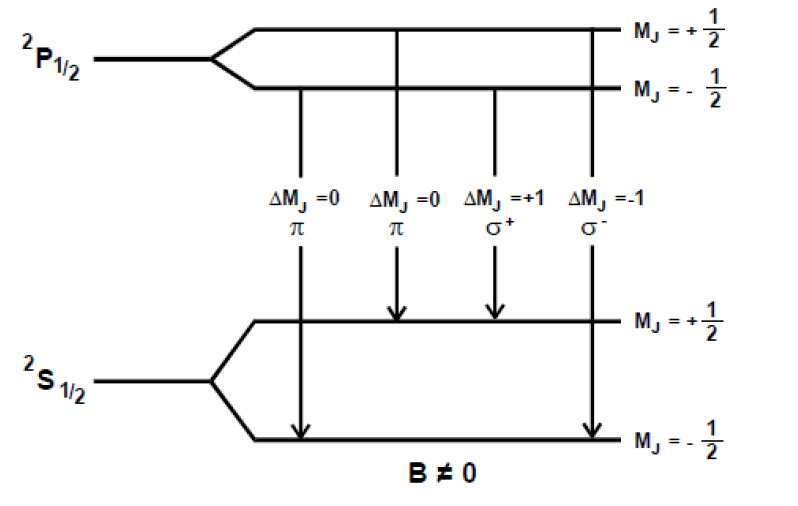
\includegraphics[width=\textwidth]{images/zeeman.png}
	\captionof{figure}{Zeeman-Aufspaltung der Energieniveaus und mögliche Übergänge [1]}
	\label{fig:zeeman}
\end{center}

\subsection{Drehimpuls und magnetisches Moment}
\begin{figure}[H]
\begin{minipage}[t]{0.38\textwidth}
\vspace{0pt}
\centering
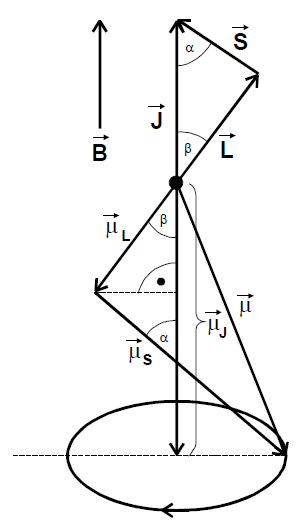
\includegraphics[width=\textwidth]{images/veranschaulichungdrehimpuls.png}
\caption{Veranschaulichung der Zusammenhänge zwischen Drehimpulsen und magn. Momenten [1]}
\label{fig:veranschaulichungdrehimpuls}
\end{minipage}
\hfill
\begin{minipage}[t]{0.6\textwidth}
\vspace{0pt}
Der Gesamtdrehimpuls $\vec{J}$ der Elektronenhülle ist mit einem magnetischen Moment $\vec{\mu}_J$ gekoppelt. Der Zusammenhang ist durch
\begin{align}
\vec{\mu}_J=-g_J\mu_B \vec{J}
\end{align}
gegeben. Es ist dabei $\mu_B$ das Bohrsche Magneton und $g_J$ der Landé-Faktor.\\
Da $\vec{\mu}_J$ um die $\vec{J}$-Achse präzediert, sind nur die Komponenten $\vec{\mu}_J  	\parallel  \vec{J}$ relevant, da die senkrechte Komponente sich heraus mittelt. Die Zusammenhänge zwischen den Drehimpulsen werden in Abbildung \ref{fig:veranschaulichungdrehimpuls} veranschaulicht.
Es lässt sich für den Landé-Faktor $g_J$ der Ausdruck
\begin{align}
g_J= \frac{\left(1+g_S\right)\left(J^2+J\right) \left(g_S-1\right)\left(S^2+S-L^2-L\right)}{2J\left(J+1\right)}
\end{align}
durch die Anwendung des Kosinus-Theorems herleiten.\\
Das Anlegen eines Magnetfeldes $\vec{B}$ führt zu einer Wechselwirkung zwischen $\vec{\mu}_J$ und $\vec{B}$ mit der Energie
\begin{align}
U_\text{mag}=-\vec{\mu}_J\dot{\vec{B}} \hspace{0.2cm}\text{.}
\end{align}
\end{minipage}
\end{figure}
Die Wechselwirkungsenergie kann aufgrund der Richtungsquantelung nur diskrete Werte
\begin{align}
U_\text{mag}=M_J g_j\mu_B B \hspace{0.2cm}\text{mit} \hspace{0.2cm}M_J \in  \left[-L,L\right]\in \mathbb{Z}
\end{align}
annehmen.\\
Jedes Energieniveau spaltet folglich in $2J+1$ Unterniveaus auf. Dies wird auch als Zeeman-Effekt bezeichnet.
\subsection{Hyperfeinstruktur}
Besitzt ein Kern einen Kernspin $I\ne 0$, so Spalten die Energieniveaus weiter in die Hyperfeinstruktur auf.\\
Es koppelt der Gesamtdrehimpuls der Elektronen $\vec{J}$ und der Kernspin $\vec{I}$ zu einen Gesamtspin
\begin{align}
\vec{F}=\vec{J}+\vec{I} \hspace{0.2cm}\text{.}
\label{eq:gesamtdrehimpuls}
\end{align}
Die dazugehörige Quantenzahl $F$ läuft dabei von $I+J$ bis $\left| I-J\right|$. Der zu $F$ gehörige Landé-Faktor $g_F$ ist durch
\begin{align}
g_F\approx g_J\frac{F\left(F+1\right)+J\left(J+1\right)+I\left(I+1\right)}{2F\left(F+1\right)}
\label{eq:landefaktoren}
\end{align}
gegeben.\\
In Abbildung \ref{fig:hyperfeinaufspaltungbeispiel} ist die Hyperfeinaufspaltung der Niveaus für ein Alkali-Atoms mit Kernspin $I = 3/2$ in zwei Unterniveaus dargestellt.
\begin{figure}[H]
\centering
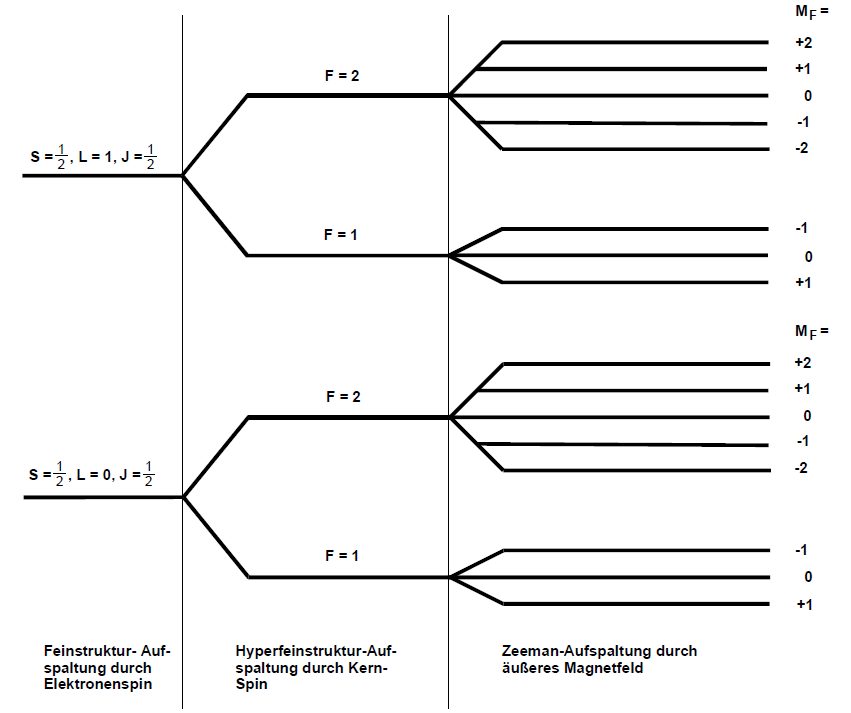
\includegraphics[width=\textwidth]{images/aufspaltunghyperfein.png}
\caption{Hyperfeinstruktur- und Zeeman-Aufspaltung der Energieniveaus eines Alkali-Atoms mit Kernspin $I = 3/2$ [1]}
\label{fig:hyperfeinaufspaltungbeispiel}
\end{figure}

\subsection{Prinzip des optischen Pumpen}
Die Auswahlregel $\Delta$M$_J\in[-1,0,1]$ impliziert vier Übergänge, die sich in Polarisation und Energie unterscheiden. Ein $\sigma^+$-Übergang beschreibt rechtszirkular-polarisiertes Licht ($\Delta$M$_J$=+1) und ein $\sigma^-$-Übergang lichtszirkular-polarisiertes Licht ($\Delta$M$_J$=-1). Ein $\pi$-Übergang beschreibt die Emission und Absorption linear polarisierten Lichtes ($\Delta$M$_J$=0). Den Grundzustand stellt das $^2$S$_{1/2}$-Niveau dar, wobei aufgrund der Boltzmann-Verteilung das M$_J=+\frac{1}{2}$-Niveau schwächer als das M$_J=-\frac{1}{2}$-Niveau besetzt sein wird. \\
Wenn nun die Probe mit $\sigma^+$-polarisiertem Licht bestrahlt wird, ist nur der Übergang von $^2$S$_{1/2}$ mit M$_J=-\frac{1}{2}$ möglich. Der angeregte Zustand geht dann durch spontane Emission in die beiden Grundzustände mit M$_J=\pm\frac{1}{2}$ über, wobei für die Relaxationszeit $\tau=10^{-8}\si{s}$ gilt.

\subsection{Verhalten bei Magnetfeld Null}

\subsection{Quadratischer Zeeman-Effekt}


\section{Aufbau}
Der Aufbau der Messapparatur ist in Abbildung \ref{fig:messaufbau} dargestellt. 
\begin{center}
	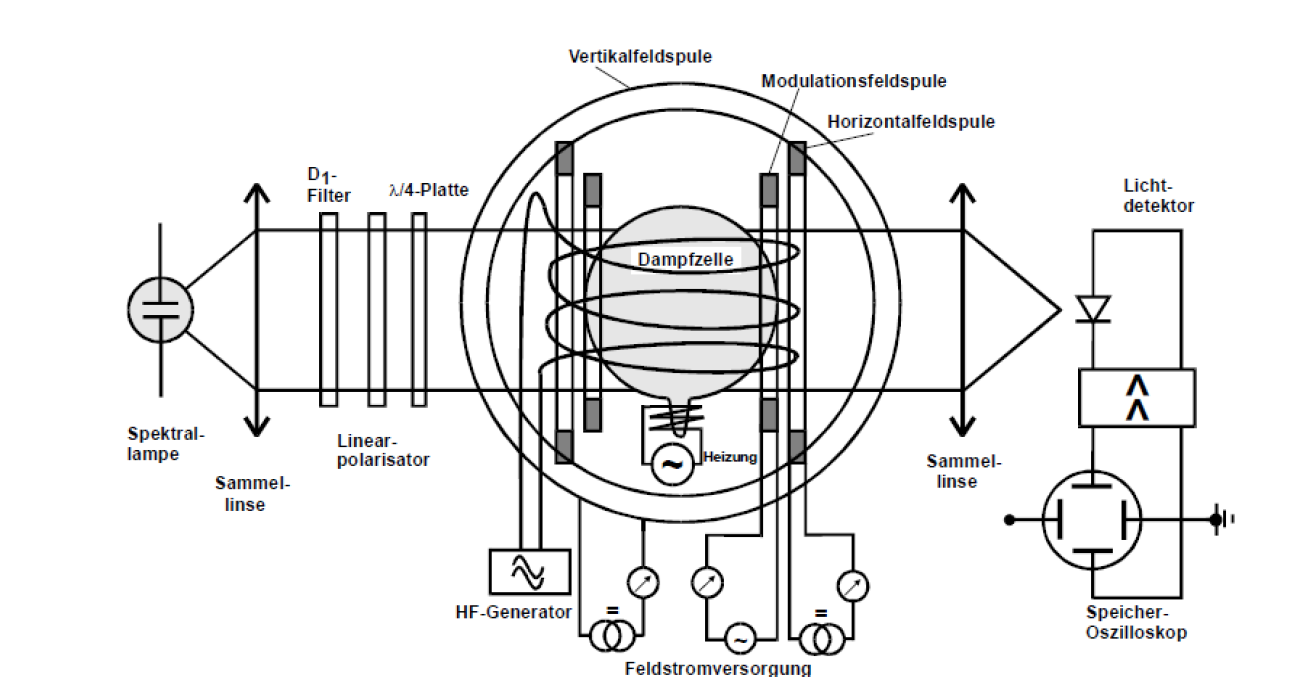
\includegraphics[width=10cm]{images/messaufbau.png}
	\captionof{figure}{Aufbau der Messapparatur, Seitenansicht}
	\label{fig:messaufbau}
\end{center}
Das Licht der Lichtquelle wird zunächst mithilfe einer Sammellinse fokussiert und dann zirkular polarisiert, bevor es auf die Dampfzelle fällt. Die Dampfzelle ist von 3 Helmholtzspulen-Paaren umgeben, die Vertikal-, Horizontal- und Modulationsspulen, die das jeweilige Magnetfeld erzeugen. \\
Der Heizofen für die Dampfzelle muss eine halbe Stunde vor Beginn der Messung eingeschalten werden, damit der optimale Dampfdruck in der Dampfzelle herrscht. Mithilfe eines Lichtdetektors können dann Schwankungen in der Intensität mittels eines Oszilloskopes dargestellt werden. \\
Zur Vorbereitung des Versuches muss die gesamte Apparatur in Nord-Süd-Richtung des Erdmagnetfeldes ausgerichtet werden, sodass das Feld der Horizontalspulen parallel bzw. antiparallel zur Horizontalkomponente des Erdmagnetfeldes steht. \\
Die technischen Daten der Spulen, die später für die Auswertung benötigt werden, sind in Tabelle \ref{tab:techdat} dargestellt. Der maximale Strom bei der Sweep- und Vertikalfeld-Spule beträgt 1 A. Mit dem Potentiometer lässt sich dieser mit 0,1 A pro Umdrehung einstellen. Der Maximalstrom bei der Horizontalfeld-Spule beträgt 3 A und kann mit 0,3 A pro Umdrehung am Potentiometer eingestellt werden.
\begin{center}
	\begin{tabular}{|c|c|c|}
		\hline Spule & Radius R [cm] & Windungen N \\
		\hline Vertikal & 11.375 & 20 \\
		\hline Modulation & 16.39 & 11 \\
		\hline Horizontal & 15.79 & 154 \\
		\hline
	\end{tabular}
\captionof{table}{Technische Daten der verwendeten Spulen}
\label{tab:techdat}
\end{center}

\section{Durchführung}
\begin{itemize}
	\item Der Strahlengang ist mithilfe der optischen Hilfsmittel so zu justieren, dass die Intensität am Detektor maximal ist. Daraufhin wird die Messapparatur mithilfe einer schwarzen Decke verhüllt. 
	\item Durch Einsatz der Vertikalspule wird das Erdmagnetfeld kompensiert. 
	\item Zur Bestimmung der Landé-Faktoren wird die Stärke des Magnetfeldes in Abhängigkeit von der Resonanzfrequenz gemesssen. Der Messbereich liegt dabei zwischen 100 kHz und 1 MHz.
	\item Aus den ermittelten Landé-Faktoren werden die Kernspins I der beiden Isotope bestimmt. 
	\item Mithilfe einer Aufnahme des Signalverlaufes wird das Isotopenverhältnis bestimmt.
	\item Die Frequenz wird nun mit einer Rechteckspannung (f=5 Hz, U${Amp}$=0-5 V) moduliert. Die Periode der entsehenden Schwingung wird in Abhängigkeit der RF-Amplitude gemessen. Mithilfe der Messwerte wird eine Hyperbelfunktion gefittet.
\end{itemize}

\section{Auswertung}

\subsection{Bestimmung der Horizontalkomponente des Erdmagnetfeldes}

\begin{center}
	\begin{tabular}{|c|c|c|}
	\hline $\nu$ [kHz] & B$_1$ [$\mu$T] & B$_2$ [$\mu$T] \\
	\hline	100	&	32.105	&	39.347	\\
	\hline	200	&	48.287	&	63.133	\\
	\hline	300	&	61.926	&	83.228	\\
	\hline	402	&	75.730	&	104.576	\\
	\hline	502	&	90.093	&	125.698	\\
	\hline	601	&	104.862	&	148.011	\\
	\hline	701	&	119.405	&	169.493	\\
	\hline	799	&	133.345	&	191.554	\\
	\hline	898	&	148.586	&	213.24	\\
	\hline	1002	&	163.310	&	234.913	\\
	\hline 
	\end{tabular}
\captionof{table}{Messwerte für das Magnetfeld im Abhängigkeit von der Resonanzfrequenz $\nu$ für induzierte Emission bei den beiden Rubidium-Isotopen}
\label{tab:magnetfeld}
\end{center}
In Tabelle \ref{tab:magnetfeld} sind die Messwerte für das gesamte horizontale Magnetfeld in Abhängigkeit von der Resonanzfrequenz für beide Rubidium-Isotope dargestellt. \\
Um die Stärke der horizontalen Komponente des Erdmagnetfeldes und die beiden Landé-Faktoren zu bestimmen, wird eine lineare Ausgleichsrechnung mit dem Ansatz
\begin{align}
f(x)=mx+b
\end{align}
durchgeführt. Die sich ergebenden Plots sind in Abbildung \ref{fig:plot1} dargestellt.
\begin{center}
	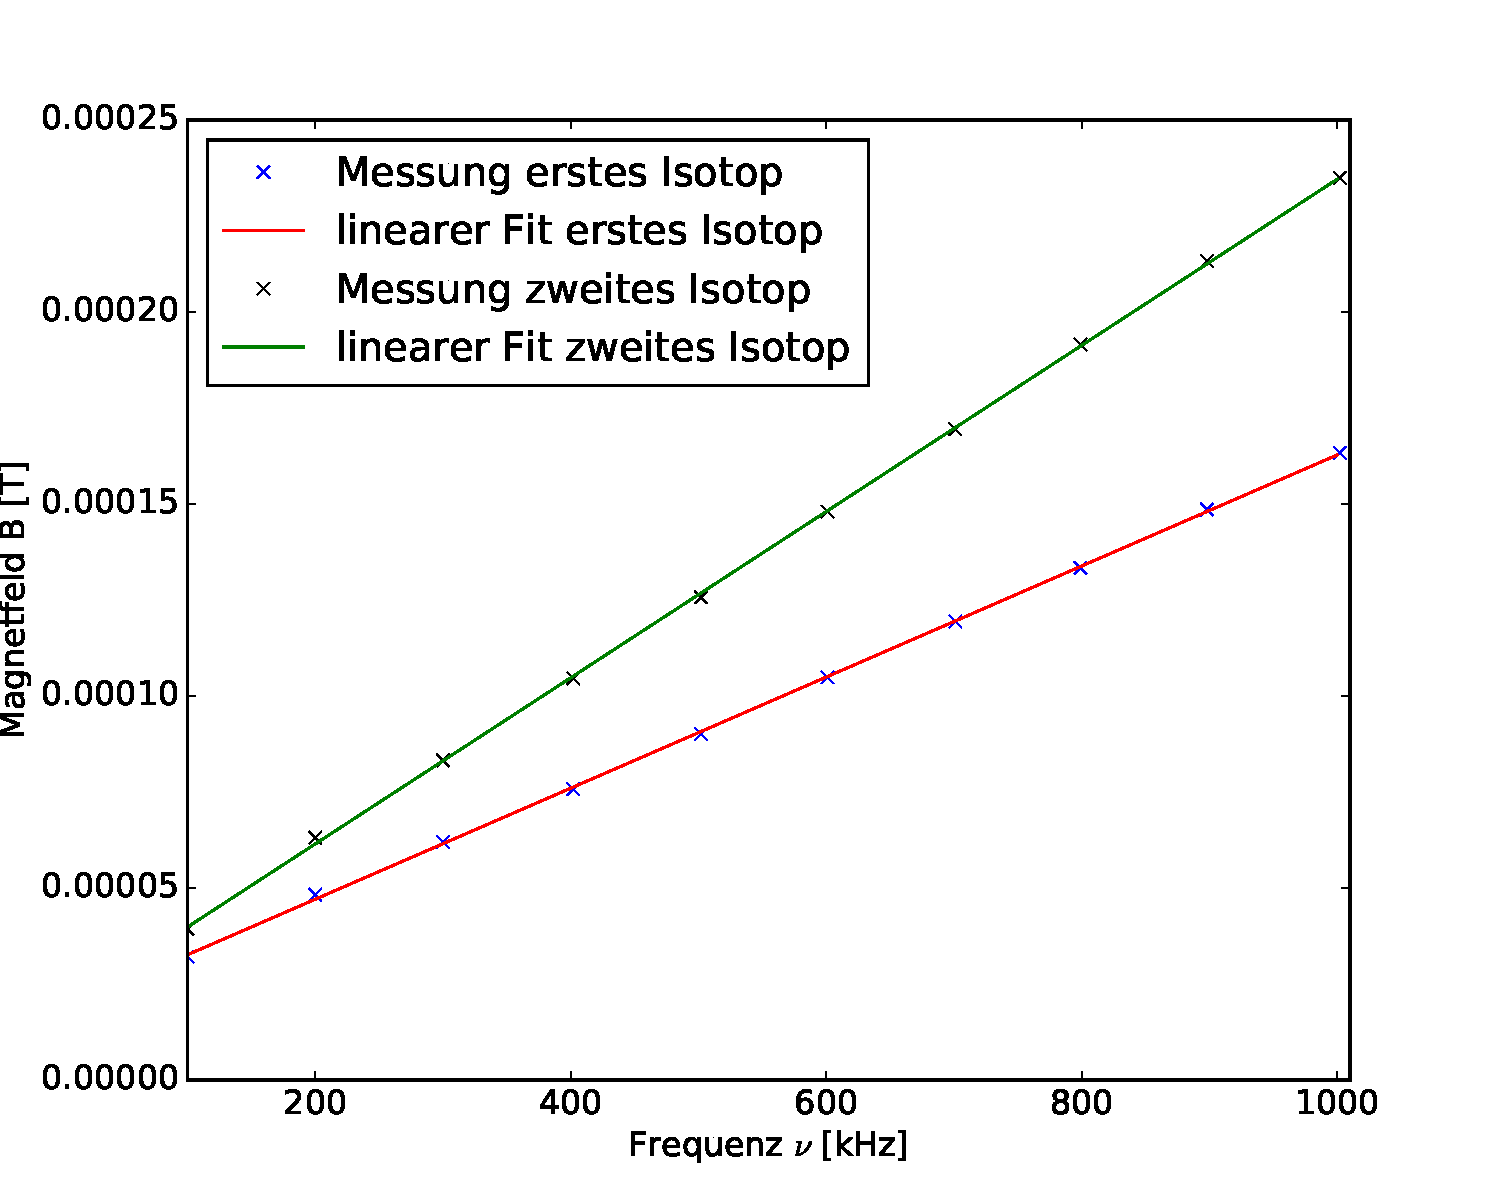
\includegraphics[width=10cm]{images/plot1.pdf}
	\captionof{figure}{Messwerte des horizontalen Magnetfeldes in Abhängigkeit der Resonanzfrequenz und linearer Fit}
	\label{fig:plot1}
\end{center}
Es ergeben sich somit folgende Fitparameter:
\begin{align*}
m_1&=(1.446\cdot 10^{-7} \pm 6.9552\cdot 10^{-10})\,\frac{\text{T}}{\text{kHz}} & m_2&=(2.164\cdot 10^{-7} \pm 9.216\cdot 10^{-10})\,\frac{\text{T}}{\text{kHz}} \\
b_1&=(1.814\cdot 10^{-5} \pm 4.318\cdot 10^{-7})\,\text{T} & b_2&=(1.819\cdot 10^{-5} \pm 5.722\cdot 10^{-7})\,\text{T}\,.
\end{align*}
Der Mittelwert der b$_i$ ergibt die Stärke der horizontalen Komponente des Erdmagnetfeldes B$_{\text{horiz}}=(1.817\pm0.022)\cdot10^{-5}$\,T. \\

\subsection{Bestimmung der Landé-Faktoren}
Mit $m=\frac{B}{\nu}$ Gleichung X und dem Wert m$_0=9.109\cdot10^{-31}$ ergeben sich somit die beiden Landé-Faktoren zu
\begin{align*}
g_{f_{1}}= 0.494 \pm 0.002\\
g_{f_{2}}= 0.331 \pm 0.001 \\
\end{align*}
Die Fehlerrechnung wurde mit dem Python-Paket \textit{uncertainties} durchgeführt.

\subsection{Bestimmung der Kernspins}
Mit Gleichung \ref{eq:gesamtdrehimpuls} und Gleichung \ref{eq:landefaktoren} sowie den zuvor bestimmten Landé-Faktoren ergeben sich mit J=1/2 die Kernspins
\begin{align}
I=-\left( 1-\frac{g_j}{4g_f}\right) +\sqrt{\left( 1-\frac{g_j}{4g_f}\right)^2-\frac{3}{4}\left( 1-\frac{g_j}{g_f}\right)}\,.
\label{eq:kernspins}
\end{align}
Mit $g_j=2.002$ ergeben sich aus Gleichung \ref{eq:kernspins} die Kernspins
\begin{align*}
I_1= 1.526 \pm 0.010\\
I_2= 2.532 \pm 0.013\,.\\
\end{align*}
Somit ist Isotop  als $^{87}$Rb mit Kernspin von I=1.5 zu identifizieren, Isotop 2 ist das Isotop $^{85}$Rb.

\subsection{Isotopenverhältnis}
Das Isotopenverhältnis kann aus dem Amplitudenverhältnis in Abbildung \ref{fig:amplituden} berechnet werden.
\begin{center}
	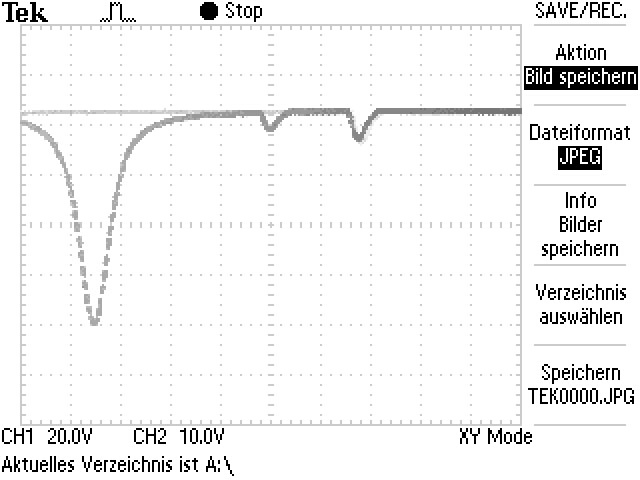
\includegraphics[width=10cm]{images/Isotopenverhaeltnis.JPG}
	\captionof{figure}{Darstellung der aufgenommenen Amplituden}
	\label{fig:amplituden}
\end{center}
Das Isotopenverhältnis ergibt sich somit zu
\begin{align*}
\frac{N(^{87}Rb)}{N(^{85}Rb)}\approx0.530\,.
\end{align*}

\subsection{Abschätzung des quadratischen Zeeman-Effektes}
Das maximal anliegende Magnetfeld liegt bei $2.3\cdot10^{-4}$\,T. Eingesetzt in Gleichung \ref{eq:quadratzeeman} ergibt sich ein Korrekturterm mit der Größenordnung $10^{-32}$\,J. Dies ist um vier Grö\ss enordnungen kleiner als der lineare Term. Somit kann der quadratische Zeeman-Effekt vernachlässigt werden. 

\subsection{Bestimmung des Verhältnisses b($^{87}$Rb)/b($^{85}$Rb)}
Die Periodendauern sind in Abhängigkeit von der anliegenden Spannung in Tabelle \ref{tab:periodendauer} dargestellt. 
\begin{center}
	\begin{tabular}{|c|c|c|}
	\hline U [V] & T$_1$ [ms] & T$_2$ [ms] \\
	\hline	1	&	2,16	&	3,18	\\
	\hline	3	&	0,72	&	1,08	\\
	\hline	5	&	0,47	&	0,64	\\
	\hline	7	&	0,32	&	0,5	\\
	\hline	9	&	0,27	&	0,42	\\
	\hline	2	&	1,12	&	1,64	\\
	\hline	4	&	0,56	&	0,8	\\
	\hline	6	&	0,38	&	0,58	\\
	\hline	8	&	0,28	&	0,44	\\
	\hline 
	\end{tabular}
\captionof{table}{Messwerte für die Periodendauer der beobachteten Schwingungen bei den beiden Rubidium-Isotopen in Abhängigkeit von der angelegten Spannung}
\label{tab:periodendauer}
\end{center}
Mit den Messdaten wird eine hyperbolische Funktion der Form
\begin{align*}
f(x)=a+\frac{b}{x+c}
\end{align*}
angepasst. Dies wird für beide Isotope durchgeführt, eine graphische Darstellung ist in Abbildung \ref{fig:periodendauer} dargestellt.
\begin{center}
	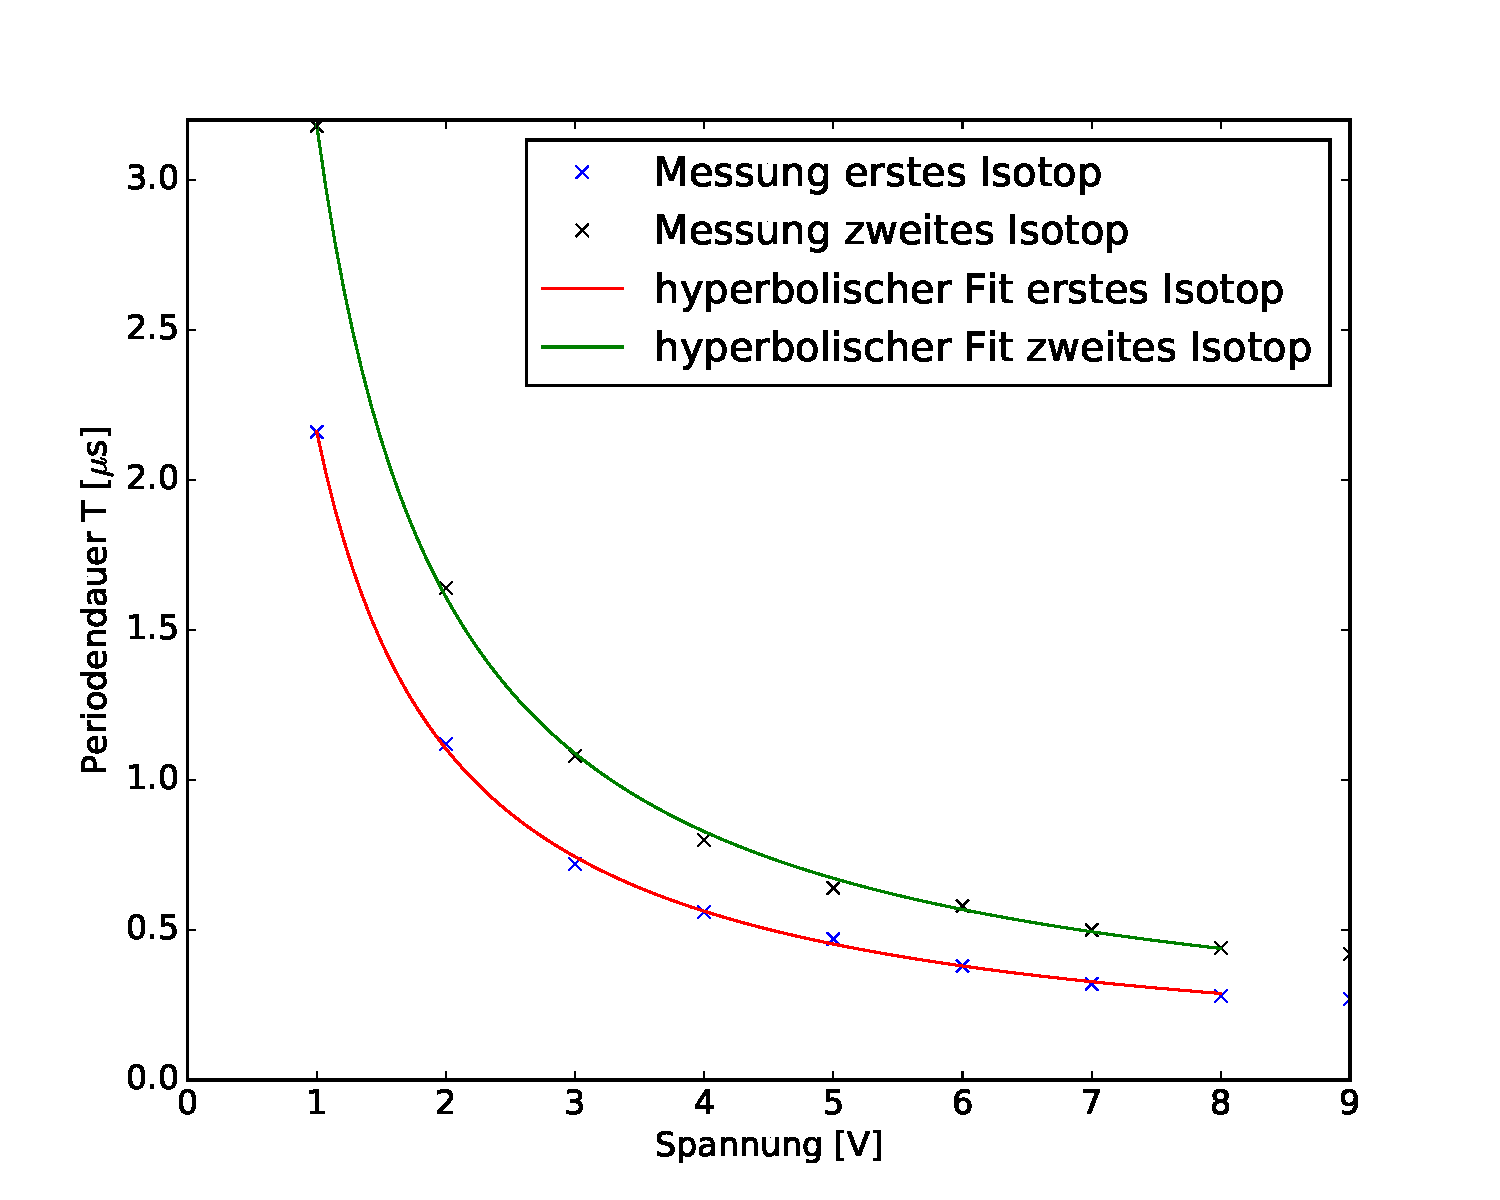
\includegraphics[width=10cm]{images/plot2.pdf}
	\captionof{figure}{Periodendauern der dargestellten Schwingungen in Abhängigkeit von der angelegten Spannung}
	\label{fig:periodendauer}
\end{center}
Die nicht-lineare Ausgleichsrechnung, durchgeführt mit Python, liefert die Fitparameter
\begin{align*}
a_1=(0.012 \pm 0.016)\,\text{ms} & a_2=(0.050 \pm 0.025)\,\text{ms} \\
b_1=(2.222 \pm 0.091)\, \text{V ms} & b_2=(3.108 \pm 0.140)\, \text{V ms} \\
c_1=(0.034 \pm 0.091)\, \text{V} & c_1=(-0.008 \pm 0.040)\, \text{V}\,.
\end{align*}
Somit ergibt sich für das gesuchte Verhältnis
\begin{align*}
\frac{b(^{87}Rb)}{b(^{85}Rb)}\approx 0.71 \pm 0.04\,.
\end{align*}
\section{Diskussion}
Der Wert der horizontalen Komponente des Erdmagnetfeldes liegt mit $18.17\,\mu$T sehr in der Nähe des erwarteten Wertes von 20$\,\mu$T. \\
Die Landé-Faktoren und die Kernspins ergeben sich im Rahmen der Messungenauigkeit zu den erwarteten Werten, wobei die Kernspins die erwarteten Werte von 1.5 bzw. 2.5 fast genau treffen. \\
Dies bestätigt die Genauigkeit des Verfahrens des optischen Pumpens. \\
Das Verhältnis der b-Werte liegt mit 0.71 deutlich unter dem erwarteten Wert, die Abweichung zum Theoriewert von 1.5 ist dabei höher als der angegebene Fehler.

\section{Quellen}
{[1]} Versuchsanleitung zu Versuch 21: \\
http://129.217.
224.2/HOMEPAGE/PHYSIKER/MASTER/SKRIPT/V21.pdf (letzte Version vom 01.08.2016, 15:30)\\
{[2]} http://www.internetchemie.info/chemiewiki/index.php?title=Rubidium-Isotope \\
{[3]} http://physics.nist.gov/PhysRefData


\end{document}